\sepframe{III. Gradient Surrogates}

\begin{frame}
\centering
So far:
\begin{itemize}
    \item Tackled \textbf{expected loss} in a \textbf{stochastic
        computation graph}
        $$ \EE_{\parser} \big[ L(\z) \big] $$
    \item<2-> Optimized with the \textbf{REINFORCE} estimator.
    \item<3-> Struggled with variance \& sampling.
\end{itemize}
\vspace{\baselineskip}
\uncover<4->{In this section:}
\begin{itemize}
    \item<4-> Consider the \textbf{deterministic alternative}:\\
        \uncover<5->{
\parbox{.333\textwidth}{\quad pick ``best'' structure}%
\parbox{.333\textwidth}{\hfil$\hat{\z}(x) \defeq \argmax_{\z \in
\mathcal{M}} \parser $\hfil}
\parbox{.333\textwidth}{}%
}
        \uncover<6->{

\parbox{.333\textwidth}{\quad incur loss}%
\parbox{.333\textwidth}{\hfil$L\big(\hat{\z}(x)\big)$\hfil}%
\parbox{.333\textwidth}{}%
}
    \item<7-> 3A: try to optimize the deterministic loss directly
    \item<8-> 3B: use this strategy to reduce variance in the stochastic model.
\end{itemize}
\end{frame}

\begin{frame}%
\frametitle{Recap: The argmax problem}
\centering%
\begin{tikzpicture}%
%
\drawcs\drawscores\drawargmax[\z]
%
\node at (0, -1) {$\frac{\partial \z}{\partial \s}=\bs{0}$};
\node[anchor=south,align=center] at (-6, \vecheight*2+1) (in) {\phantom{input}};
\node[anchor=south,align=center] at (6, \vecheight*2+1) (out) {\phantom{output}};
\end{tikzpicture}%
\\[-\baselineskip]

\begin{tikzpicture}[overlay]
    \draw[axisline,->] (3, 3) -- (3, 6) node[left] {$\zz_1$};
    \draw[axisline,->] (3, 3) -- (7, 3) node[right]{$\ss_1$};

    \node[axislabel,left] at (3, 3) {$0$};
    \node[axislabel,left] at (3, 5) {$1$};

    \draw[axisline] ($(3,3) + (-\ticksize, 0)$) -- ($(3,3) + (+\ticksize, 0)$);
    \draw[axisline] ($(3,4) + (-\ticksize, 0)$) -- ($(3,4) + (+\ticksize, 0)$);
    \draw[axisline] ($(3,5) + (-\ticksize, 0)$) -- ($(3,5) + (+\ticksize, 0)$);

    \draw[axisline] ($(3,3) + (0, -\ticksize)$) -- ($(3,3) + (0, +\ticksize)$);
    \draw[axisline] ($(4,3) + (0, -\ticksize)$) -- ($(4,3) + (0, +\ticksize)$);
    \draw[axisline] ($(5,3) + (0, -\ticksize)$) -- ($(5,3) + (0, +\ticksize)$);
    \draw[axisline] ($(6,3) + (0, -\ticksize)$) -- ($(6,3) + (0, +\ticksize)$);

    \node[axislabel,below] at (4, 3) {$\ss_2 - 1$};
    \node[axislabel,below] at (5, 3) {$\ss_2$};
    \node[axislabel,below] at (6, 3) {$\ss_2 + 1$};

    \draw[ultra thick,colorArgmax] (3, 3) -- (5,3) ;
    \draw[ultra thick,colorArgmax] (5, 5) -- (7,5) ;

    \node[anchor=south,align=center] at (-5, 4) (in) {$\z = \argmax(\s)$};
\end{tikzpicture}\end{frame}


\begin{frame}%
\frametitle{Softmax}
\centering%
\begin{tikzpicture}%
%
\drawcs\drawscores\drawsoftmax
\node at (0, -1) {$\frac{\partial \p}{\partial \s}=\operatorname{diag}(\p) - \p\p^\top$};
\node[anchor=south,align=center] at (-6, \vecheight*2+1) (in) {\phantom{input}};
\node[anchor=south,align=center] at (6, \vecheight*2+1) (out) {\phantom{output}};
\end{tikzpicture}
\\[-\baselineskip]

\begin{tikzpicture}[overlay]
    \draw[axisline,->] (3, 3) -- (3, 6) node[left] {$\pp_1$};
    \draw[axisline,->] (3, 3) -- (7, 3) node[right]{$\ss_1$};

    \node[axislabel,left] at (3, 3) {$0$};
    \node[axislabel,left] at (3, 5) {$1$};

    \draw[axisline] ($(3,3) + (-\ticksize, 0)$) -- ($(3,3) + (+\ticksize, 0)$);
    \draw[axisline] ($(3,4) + (-\ticksize, 0)$) -- ($(3,4) + (+\ticksize, 0)$);
    \draw[axisline] ($(3,5) + (-\ticksize, 0)$) -- ($(3,5) + (+\ticksize, 0)$);

    \draw[axisline] ($(3,3) + (0, -\ticksize)$) -- ($(3,3) + (0, +\ticksize)$);
    \draw[axisline] ($(4,3) + (0, -\ticksize)$) -- ($(4,3) + (0, +\ticksize)$);
    \draw[axisline] ($(5,3) + (0, -\ticksize)$) -- ($(5,3) + (0, +\ticksize)$);
    \draw[axisline] ($(6,3) + (0, -\ticksize)$) -- ($(6,3) + (0, +\ticksize)$);

    \node[axislabel,below] at (4, 3) {$\ss_2 - 1$};
    \node[axislabel,below] at (5, 3) {$\ss_2$};
    \node[axislabel,below] at (6, 3) {$\ss_2 + 1$};

    \draw[ultra thick,colorArgmax] (3, 3) -- (5,3) ;
    \draw[ultra thick,colorArgmax] (5, 5) -- (7,5) ;

    \draw (3, 3.1) edge[colorSoftmax,ultra thick,out=360,in=180,looseness=1.5] (7, 4.9);

    \node[anchor=south,align=center] at (-5, 4) (in) {$\pp_j = \exp(\ss_j) / Z$};

\end{tikzpicture}%
\end{frame}



\begin{frame}%
\frametitle{Straight-Through Estimator}%
\cornercite{hinton2012ste,bengio2013ste}%
\makebox[\textwidth][c] {% two boxes
\begin{minipage}[t][][c]{.66\textwidth}
\begin{itemize}%
\item<2-> \underline{Forward}: $\z=\argmax(\s)$
\item<4-> \underline{Backward}:
pretend $\z$ was some continuous $\tilde\p$; $\pfrac{\tilde{\p}}{\s}\neq \bs{0}$
\begin{itemize}
\item<6-> simplest: identity, $\tilde\p(\s)=\s, \pfrac{\tilde \p}{\s}=\bs{I}$
\item<7-> others, e.g.\ softmax $\tilde\p(\s) = \softmax(\s), \pfrac{\tilde\p}{\s}=\diag(\tilde\p) - \tilde\p\tilde\p^\top$
\end{itemize}%
\item<8-> More explanation in a while

\end{itemize}%
\end{minipage}%
% \hfill%
%
\begin{minipage}[t][][c]{.33\textwidth}
\centering
\begin{tikzpicture}
{
\node[anchor=south] at (-.3-.5*\vecwidth, \vecheight*5+.3) {$\s$};
\draw[elem,fill=vecfg!60!vecbg] (-1-\vecwidth, \vecheight*4+1) rectangle (-1, \vecheight*5+1);
\draw[elem,fill=vecfg!85!vecbg] (-1-\vecwidth, \vecheight*3+1) rectangle (-1, \vecheight*4+1);
\draw[elem,fill=vecfg!60!vecbg] (-1-\vecwidth, \vecheight*2+1) rectangle (-1, \vecheight*3+1);
\draw[elem,fill=vecfg!75!vecbg] (-1-\vecwidth, \vecheight*1+1) rectangle (-1, \vecheight*2+1);
\draw[elem,fill=vecfg!50!vecbg] (-1-\vecwidth, \vecheight*0+1) rectangle (-1, \vecheight*1+1);
}(nodetilde)

% {}
\uncover<2->{
\def\vecwidth{.5}
\def\vecheight{.5}
% \drawargmax
{
\node[anchor=south] at (1.5+.5*\vecwidth, \vecheight*9.6) {$\z$};
\draw[elem,fill=vecfg! 0!vecbg]  (1, \vecheight*4+3) rectangle (1+\vecwidth, \vecheight*5+3);
\draw[elem,fill=vecfg!70!vecbg]  (1, \vecheight*3+3) rectangle (1+\vecwidth, \vecheight*4+3);
\draw[elem,fill=vecfg! 0!vecbg]  (1, \vecheight*2+3) rectangle (1+\vecwidth, \vecheight*3+3);
\draw[elem,fill=vecfg! 0!vecbg]  (1, \vecheight*1+3) rectangle (1+\vecwidth, \vecheight*2+3);
\draw[elem,fill=vecfg! 0!vecbg]  (1, \vecheight*0+3) rectangle (1+\vecwidth, \vecheight*1+3);
}
}
\uncover<3->{
% Arrows forward
\draw[->][very thick, color=mygr](-2*\vecheight,6*\vecheight) -- (2*\vecheight,8.5*\vecheight);
\draw[->][very thick, color=mygr](3*\vecheight,8.5*\vecheight) -- (5*\vecheight,8.5*\vecheight);
\draw[->][very thick, color=mygr](-5*\vecheight,6*\vecheight) -- (-3.5*\vecheight,6*\vecheight);
}
\uncover<4->{
\node[anchor=south] at (1.5+.5*\vecwidth, \vecheight*5-0.8) {$\tilde \p$};
\draw[elem,fill=vecfg!30!vecbg]  (1, \vecheight*4) rectangle (1+\vecwidth, \vecheight*5);
\draw[elem,fill=vecfg!50!vecbg]  (1, \vecheight*3) rectangle (1+\vecwidth, \vecheight*4);
\draw[elem,fill=vecfg!35!vecbg]  (1, \vecheight*2) rectangle (1+\vecwidth, \vecheight*3);
\draw[elem,fill=vecfg!25!vecbg]  (1, \vecheight*1) rectangle (1+\vecwidth, \vecheight*2);
\draw[elem,fill=vecfg!15!vecbg]  (1, \vecheight*0) rectangle (1+\vecwidth, \vecheight*1);
}
\uncover<5->{
% arrows back
\draw[->][tGreen,very thick](2*\vecheight,2.5*\vecheight) -- (-2*\vecheight,5.5*\vecheight);
\draw[->][tGreen,very thick](5*\vecheight,2.5*\vecheight) -- (3*\vecheight,2.5*\vecheight);
\draw[->][tGreen,very thick](-3.5*\vecheight,5.5*\vecheight) -- (-5*\vecheight,5.5*\vecheight);
}

\end{tikzpicture}
\end{minipage}}
\uncover<9>{\overlaybox{What about the structured case?}}
\end{frame}

\againframe{structuretypes}

\begin{frame}%
\frametitle{STE for incremental structures}%
\centering
\begin{itemize}
    \item<2-> Build a structure as a sequence of discrete choices (e.g., shift-reduce)
    \item<3-> Assigns a score to any (partial structure, action) tuple.
    \item<4-> In this case, we just apply the straight-through estimator for each step.
    \item<5-> \underline{Forward}: the \textbf{highest scoring action} for each step
    \item<6-> \underline{Backward}: pretend that we had used a \textbf{differentiable surrogate function}
    \item[]<7-> \underline{Example}: Latent Tree Learning with Differentiable Parsers: Shift-Reduce Parsing and Chart Parsing \citep{maillard2018latent} (STE through beam search).
\end{itemize}
\end{frame}

\begin{frame}
\frametitle{STE for the factorized approach}
Requires a bit more work:
\begin{itemize}
\item Recap: marginal polytope
\item Predicting structures globally: Maximum A Posteriori (MAP)
\item Deriving Straight-Through and SPIGOT
\end{itemize}
\end{frame}

\againframe{marginalpoly}

\begin{frame}
\frametitle{Predicting structures from scores of parts}
% \centering
\begin{columns}[t]%
\begin{column}{.4\textwidth}%
\centering
\begin{itemize}
\item $\eta(i \rightarrow j)$: score of arc $i \rightarrow j$
\item $\zz(i \rightarrow j)$: is arc $i \rightarrow j$ selected?
\item<2-> Task-specific algorithm for the highest-scoring structure.
%\item<3-> Backward: identity $\frac{\partial \tilde\mg}{\partial \pr}=\bs{I}$
\end{itemize}
\end{column}
\begin{column}[T]{.6\textwidth}%
\centering
\begin{tikzpicture}
% \only<3>{\drawcs}
% \only<4->{
\node[anchor=south] at (0, \vecheight*4) {\cartoon[.5]{2/3}};
\node[anchor=south] at (0, \vecheight*2.5) {\cartoon[.5]{1/2}};
%\node[anchor=south] at (0, \vecheight*1.5) {$\cdots$};
\node[anchor=south] at (0, \vecheight*0.5) {\cartoon[.5]{1/4}};
% }
% \only<3->{%
% \drawscores
{\node[anchor=south] at (-1-.5*\vecwidth, \vecheight*5+.1) {$\pr$};
\draw[elem,fill=vecfg!60!vecbg] (-1-\vecwidth, \vecheight*4) rectangle (-1, \vecheight*5);
\draw[elem,fill=vecfg!85!vecbg] (-1-\vecwidth, \vecheight*3) rectangle (-1, \vecheight*4);
\draw[elem,fill=vecfg!60!vecbg] (-1-\vecwidth, \vecheight*2) rectangle (-1, \vecheight*3);
\draw[elem,fill=vecfg!75!vecbg] (-1-\vecwidth, \vecheight*1) rectangle (-1, \vecheight*2);
\draw[elem,fill=vecfg!50!vecbg] (-1-\vecwidth, \vecheight*0) rectangle (-1, \vecheight*1);
}
% \drawargmax
{\node[anchor=south] at (1+.5*\vecwidth, \vecheight*5+.1) {$\z$};
\draw[elem,fill=vecfg! 0!vecbg]  (1, \vecheight*4) rectangle (1+\vecwidth, \vecheight*5);
\draw[elem,fill=vecfg!70!vecbg]  (1, \vecheight*3) rectangle (1+\vecwidth, \vecheight*4);
\draw[elem,fill=vecfg! 0!vecbg]  (1, \vecheight*2) rectangle (1+\vecwidth, \vecheight*3);
\draw[elem,fill=vecfg!70!vecbg]  (1, \vecheight*1) rectangle (1+\vecwidth, \vecheight*2);
\draw[elem,fill=vecfg! 0!vecbg]  (1, \vecheight*0) rectangle (1+\vecwidth, \vecheight*1);
}


% \node[anchor=south] at (-2, \vecheight*3+1) (in-end) {};
\node[anchor=south,align=center] at (6, \vecheight*3+1)
(out){output\\$\widetilde{\bs{y}}$};
% \node[anchor=south] at (2, \vecheight*3+1) (out-end) {};
% \path (in) edge[->,very thick,bend right=50] (in-end);
\node[anchor=south] at (4, \vecheight*3+.9) (out-mid) {
    {\cartoon[.9]{1/2,1/4}}
};
\path (out-end) edge[->,very thick,bend right=50] (out-mid.south west);
\path (out-mid.south east) edge[->,very thick,bend right=50] (out);
% }
\end{tikzpicture}
\end{column}
\end{columns}
\end{frame}

\begin{frame}<1>[label=algos]
\frametitle{Algorithms for specific structures}
\fontsize{10pt}{11}\selectfont%
\centering%
\renewcommand{\arraystretch}{3}%
\begin{tabular}{l c <{\onslide<2->}c<{\onslide}}
&\textbf{Best structure (MAP)} & \textbf{Marginals} \\
\tikzmark{seq}%
\textbf{Sequence tagging}
& \makecell{Viterbi \\ \citep{Rabiner1989}}
& \makecell{Forward-Backward \\ \citep{Rabiner1989}}
\\
%
\textbf{Constituent trees}
& \makecell{CKY \\ \citep{kasami,younger} \\ \citep{cocke}}
& \makecell{Inside-Outside\\\citep{insideoutside}}%
\\
\tikzmark{alig}%
\textbf{Temporal alignments}
& \makecell{DTW \\ \citep{dtw}}
& \makecell{Soft-DTW \\ \citep{softdtw}}
\\
\textbf{Dependency trees}
& \makecell{Max. Spanning Arborescence \\ \citep{Chu1965,Edmonds1967}}
& \makecell{Matrix-Tree \\ \citep{Kirchhoff1847}}
\\
%
\textbf{Assignments}
& \makecell{Kuhn-Munkres \\ \citep{hungarian,lapjv}}
& \makecell{\alert{\#P-complete} \\ \citep{valiant,taskar-thesis}} \\
\end{tabular}
\begin{tikzpicture}[%
    remember picture,
    overlay]
    \draw<3->[decorate,decoration={brace,amplitude=5pt}] ([xshift=-1.5ex]pic cs:alig)
         -- ([xshift=-1.5ex]pic cs:seq)
         node [midway,xshift=-15pt,align=center] {dyn.\\prog.};
\end{tikzpicture}
\end{frame}


\begin{frame}[t]
\frametitle{Structured Straight-Through}
\makebox[\textwidth][c] {% two boxes
\begin{minipage}[t][][c]{.5\textwidth}
\begin{itemize}
\item Forward pass:
\\ \quad Find highest-scoring structure:
\\ \quad $\z = \displaystyle\argmax_{\z\in\ZZ} \pr^\top \z$
\item Backward pass:
\\ \quad pretend we used $\tilde\mg = \pr$.
\end{itemize}
\end{minipage}%
\begin{minipage}[t][][c]{.5\textwidth}
\centering
\begin{tikzpicture}
{
\node[anchor=south] at (-.3-.5*\vecwidth, \vecheight*5+.3) {$\pr$};
\draw[elem,fill=vecfg!60!vecbg] (-1-\vecwidth, \vecheight*4+1) rectangle (-1, \vecheight*5+1);
\draw[elem,fill=vecfg!85!vecbg] (-1-\vecwidth, \vecheight*3+1) rectangle (-1, \vecheight*4+1);
\draw[elem,fill=vecfg!60!vecbg] (-1-\vecwidth, \vecheight*2+1) rectangle (-1, \vecheight*3+1);
\draw[elem,fill=vecfg!75!vecbg] (-1-\vecwidth, \vecheight*1+1) rectangle (-1, \vecheight*2+1);
\draw[elem,fill=vecfg!50!vecbg] (-1-\vecwidth, \vecheight*0+1) rectangle (-1, \vecheight*1+1);
}(nodetilde)

\def\vecwidth{.5}
\def\vecheight{.5}
% \drawargmax
{
\node[anchor=south] at (1.5+.5*\vecwidth, \vecheight*9.6) {$\z$};
\draw[elem,fill=vecfg! 0!vecbg]  (1, \vecheight*4+3) rectangle (1+\vecwidth, \vecheight*5+3);
\draw[elem,fill=vecfg!70!vecbg]  (1, \vecheight*3+3) rectangle (1+\vecwidth, \vecheight*4+3);
\draw[elem,fill=vecfg! 0!vecbg]  (1, \vecheight*2+3) rectangle (1+\vecwidth, \vecheight*3+3);
\draw[elem,fill=vecfg! 0!vecbg]  (1, \vecheight*1+3) rectangle (1+\vecwidth, \vecheight*2+3);
\draw[elem,fill=vecfg!70!vecbg]  (1, \vecheight*0+3) rectangle (1+\vecwidth, \vecheight*1+3);
}
% Arrows forward
\draw[->][very thick, color=mygr](-2*\vecheight,6*\vecheight) -- (2*\vecheight,8.5*\vecheight);
\draw[->][very thick, color=mygr](3*\vecheight,8.5*\vecheight) -- (5*\vecheight,8.5*\vecheight);
\draw[->][very thick, color=mygr](-5*\vecheight,6*\vecheight) -- (-3.5*\vecheight,6*\vecheight);
\node[anchor=south] at (1.5+.5*\vecwidth, \vecheight*5-0.8) {$\tilde \mg$};
\draw[elem,fill=vecfg!60!vecbg]  (1, \vecheight*4) rectangle (1+\vecwidth, \vecheight*5);
\draw[elem,fill=vecfg!85!vecbg]  (1, \vecheight*3) rectangle (1+\vecwidth, \vecheight*4);
\draw[elem,fill=vecfg!60!vecbg]  (1, \vecheight*2) rectangle (1+\vecwidth, \vecheight*3);
\draw[elem,fill=vecfg!75!vecbg]  (1, \vecheight*1) rectangle (1+\vecwidth, \vecheight*2);
\draw[elem,fill=vecfg!50!vecbg]  (1, \vecheight*0) rectangle (1+\vecwidth, \vecheight*1);
% arrows back
\draw[->][tGreen,very thick](2*\vecheight,2.5*\vecheight) -- (-2*\vecheight,5.5*\vecheight);
\draw[->][tGreen,very thick](5*\vecheight,2.5*\vecheight) -- (3*\vecheight,2.5*\vecheight);
\draw[->][tGreen,very thick](-3.5*\vecheight,5.5*\vecheight) -- (-5*\vecheight,5.5*\vecheight);
\end{tikzpicture}
\end{minipage}}
\end{frame}



\begin{frame}
\frametitle{Straight-Through Estimator}
\framesubtitle{Revisited}
\begin{itemize}
\item<2-> In the forward pass, $\z = \argmax(\s)$.
\item<3-> if we had labels (multi-task learning),
$L_\text{MTL} = \textcolor{tBleu}{L\big(\hat{y}(\z), y\big)} \textcolor{tGreen}{+
L_\text{hid}(\s,\z^\text{true})}$
\item<4-> One choice: perceptron loss
\textcolor{tGreen}{$L_\text{hid}(\s,\z^\text{true}) = \s^\top\z - \s^\top
\z^\text{true};
\quad
\pfrac{L_\text{hid}}{\s} = \z - \z^\text{true}
$}.
\item<5-> We don't have labels! Induce labels by ``pulling back'' the downstream
target:
\\ \quad the ``best'' (unconstrained) latent value would be:\quad
$\argmin_{\tilde{\z}\in\mathbb{R}^D} L\big(\hat{y}(\tilde{\z}), y\big)$
\item<6-> One gradient descent step starting from $\z$: $\z^\text{true} \leftarrow
\z -  \pfrac{L}{\z}$
\item[]<7->% perceptron loss yields:
$$
\pfrac{L_\text{MTL}}{\s} =
\textcolor{tBleu}{\underbrace{\pfrac{L}{\s}}_{=\bs{0}}} +
\textcolor{tGreen}{\pfrac{L_\text{hid}}{\s}}
\uncover<8->{%
= \textcolor{tGreen}{\z - \left(\z -
\pfrac{L}{\z}
\right)
} =
\pfrac{L}{\z}
}
$$
\end{itemize}%
\cornercite{stspigotnote}%
\end{frame}


\begin{frame}%
\frametitle{Straight-Through in the structured case}%
\cornercite{peng2018backpropagating,stspigotnote}
% \centering
\begin{columns}[t]
\begin{column}{.65\textwidth}
\begin{itemize}
\small
\item<1-> Structured STE: perceptron update with induced annotation
\small
$$\argmin_{\mg \in \reals^D}
L(\hat{y}(\mg), y)
\quad\quad
\approx \z - \nabla_{\z} L(\z)
\rightarrow \z^\text{true}
$$ \\
{\small (one step of gradient descent)}
\item<2-> SPIGOT takes into account the constraints; uses the induced annotation
$$\argmin_{\mg \textcolor{tPink}{\in
\mathcal{M}}}
L(\hat{y}(\mg), y)
\quad
\approx \operatorname{Proj}_\mathcal{M} \big(\z -
\nabla_{\z} L(\z) \big)
\rightarrow \z^\text{true}
$$ \\
{\small (one step of \emph{projected} gradient descent!)}
\item<3-> We discuss a generic way to compute the projection in part 4.
\end{itemize}
\end{column}
\begin{column}[T]{.35\textwidth}
\begin{itemize}
    \item[]<1-> 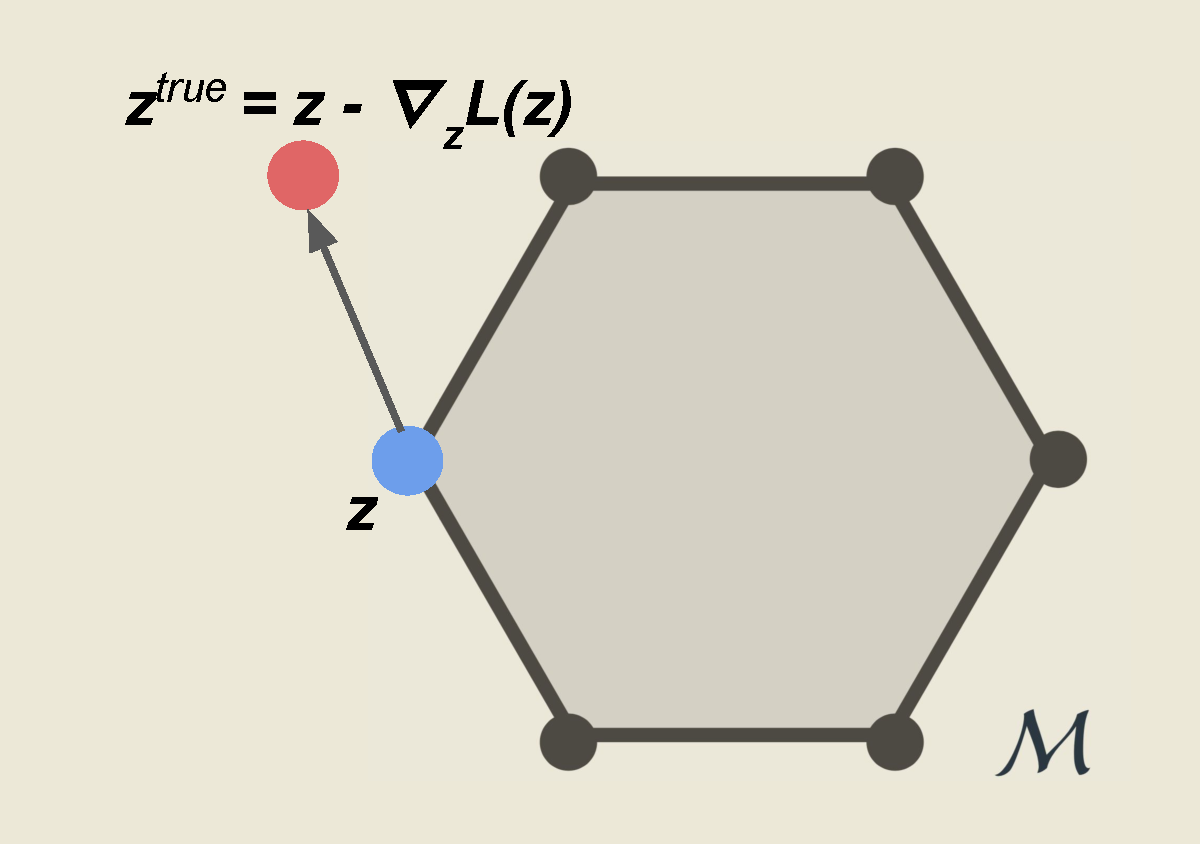
\includegraphics[width=0.8\textwidth]{img/300_spigot_ste.pdf}
    \item[]<2-> 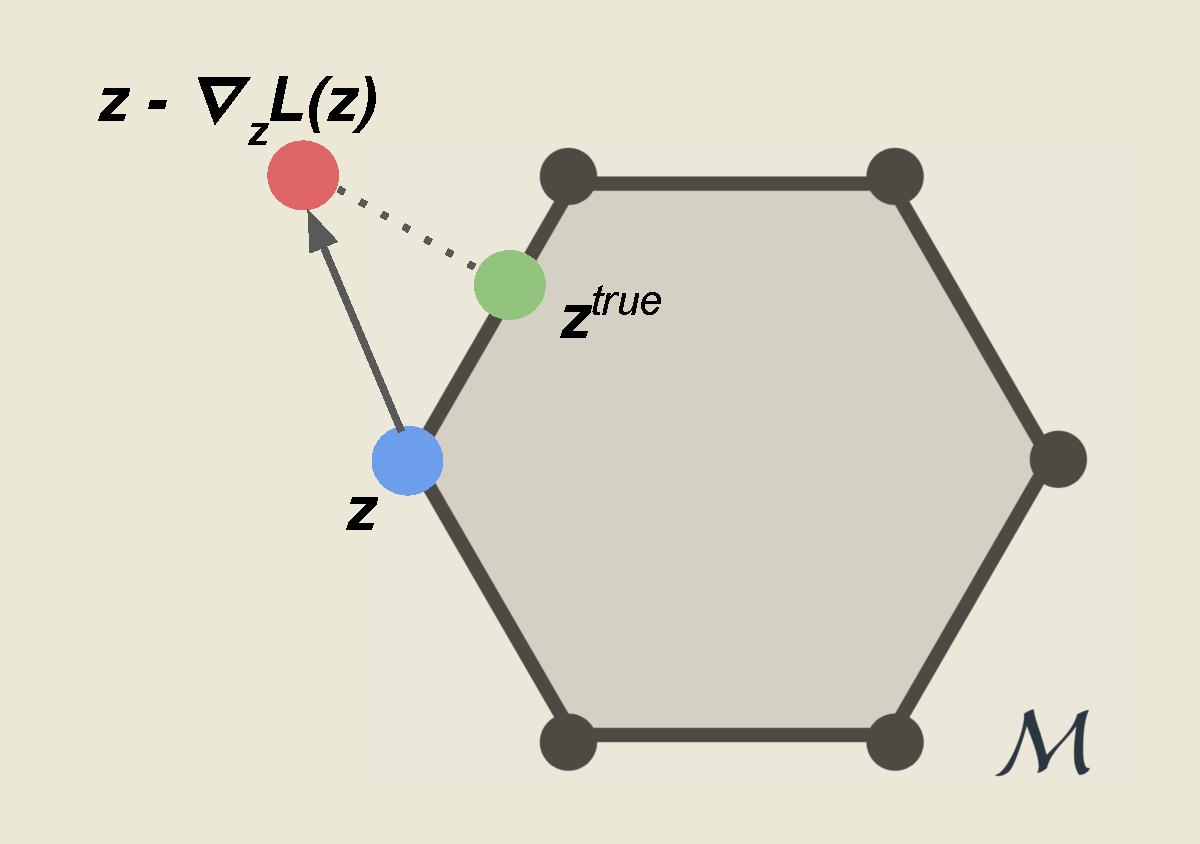
\includegraphics[width=0.8\textwidth]{img/300_spigot_update.pdf}
\end{itemize}
\end{column}
\end{columns}
\end{frame}


\begin{frame}%
\frametitle{Summary: Straight-Through Estimator}%
\centering
\begin{itemize}
    \item[]<2-> We saw how to use the \textit{Straight-Through Estimator} to allow learning models with \textit{argmax} in the middle of the computation graph.\\
    \item[]<3-> We were optimizing
\parbox{.333\textwidth}{\hfil$L\big(\hat{\z}(x)\big)$\hfil}\\

    \item[]<4->
    \smallskip
    Now we will see how to apply STE for stochastic graphs, as an alternative approach of REINFORCE.
\end{itemize}
\end{frame}


\begin{frame}%
\frametitle{Stochastic node in the computation graph}%
\centering
\begin{itemize}
    \item[]<2-> Recall the stochastic objective:
        $$ \EE_{\parser} \big[ L(\z) \big] $$
    \item<3-> REINFORCE (previous section).
    \uncover<4->{ High variance. \emoji{frown}}
    \item<5-> An alternative is using the \textit{reparameterization trick} \citep{kingma2013auto}.
\end{itemize}
\end{frame}


\begin{frame}
\frametitle{Categorical reparameterization}%
\uncover<3->{\cornercite{jang2016categorical, maddison2016concrete}}
\centering
\begin{columns}[T]
\begin{column}[T]{.5\textwidth}
\begin{itemize}
    \item<2-> Sampling from a categorical value in the middle of the computation graph.\\
    $\z \sim \parser \propto \exp \bs{s}_{\parp}(\z \mid x)$
    \item<3-> What is the gradient of a sample $\pfrac{\z}{\parp}$?!
    \item<4-> Reparameterization:
    Move the stochasticity out of the gradient path.
    \item<5-> Makes $\z$ deterministic w.r.t.\ $\s$!

\end{itemize}
\end{column}
\begin{column}{.6\textwidth}
\only<2-3>{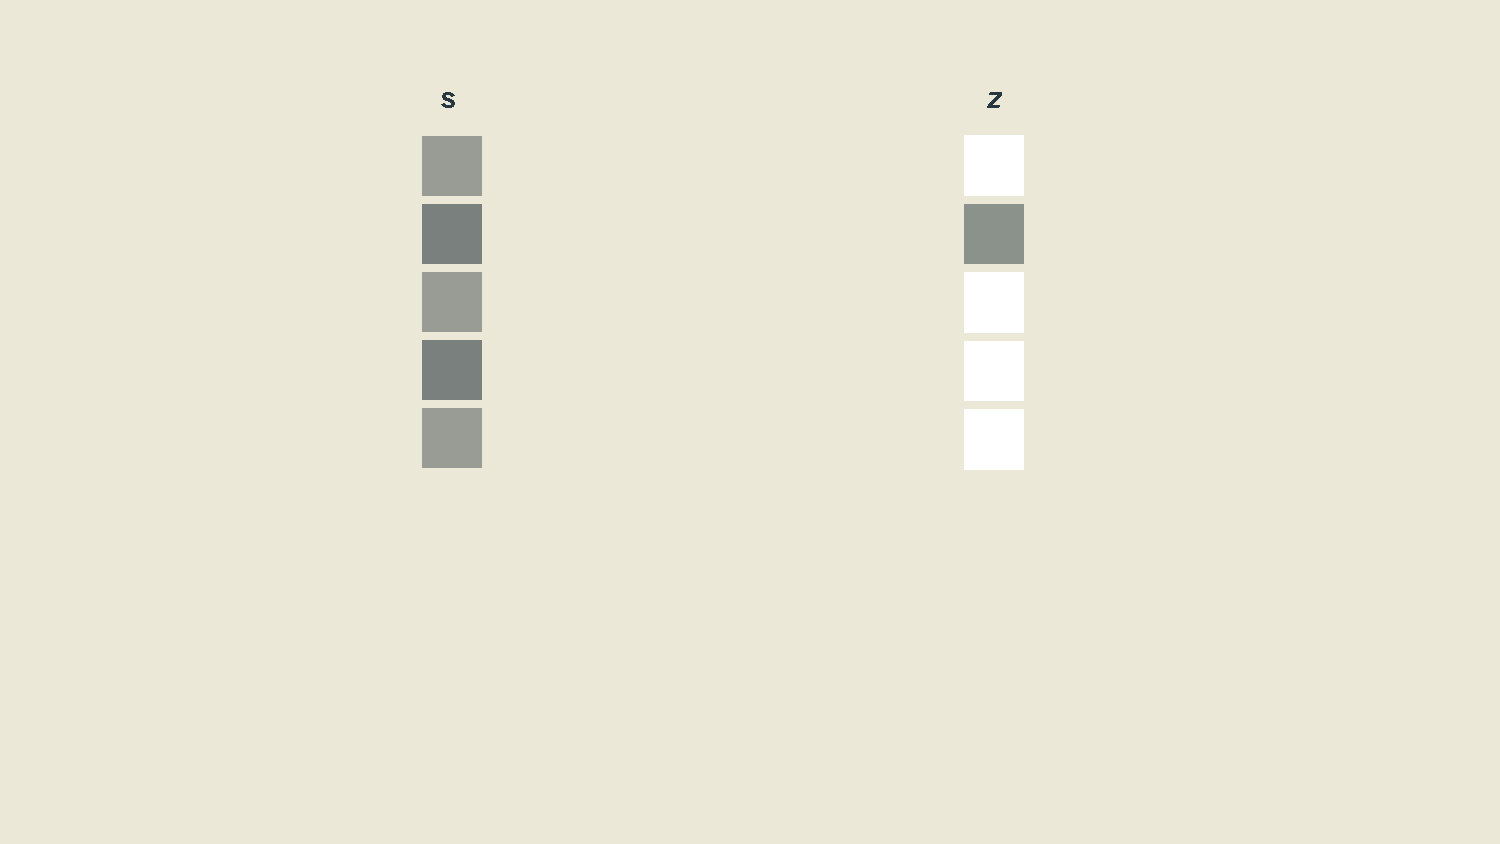
\includegraphics[width=\textwidth]{img/300_reparam_1.pdf}}
\only<4>{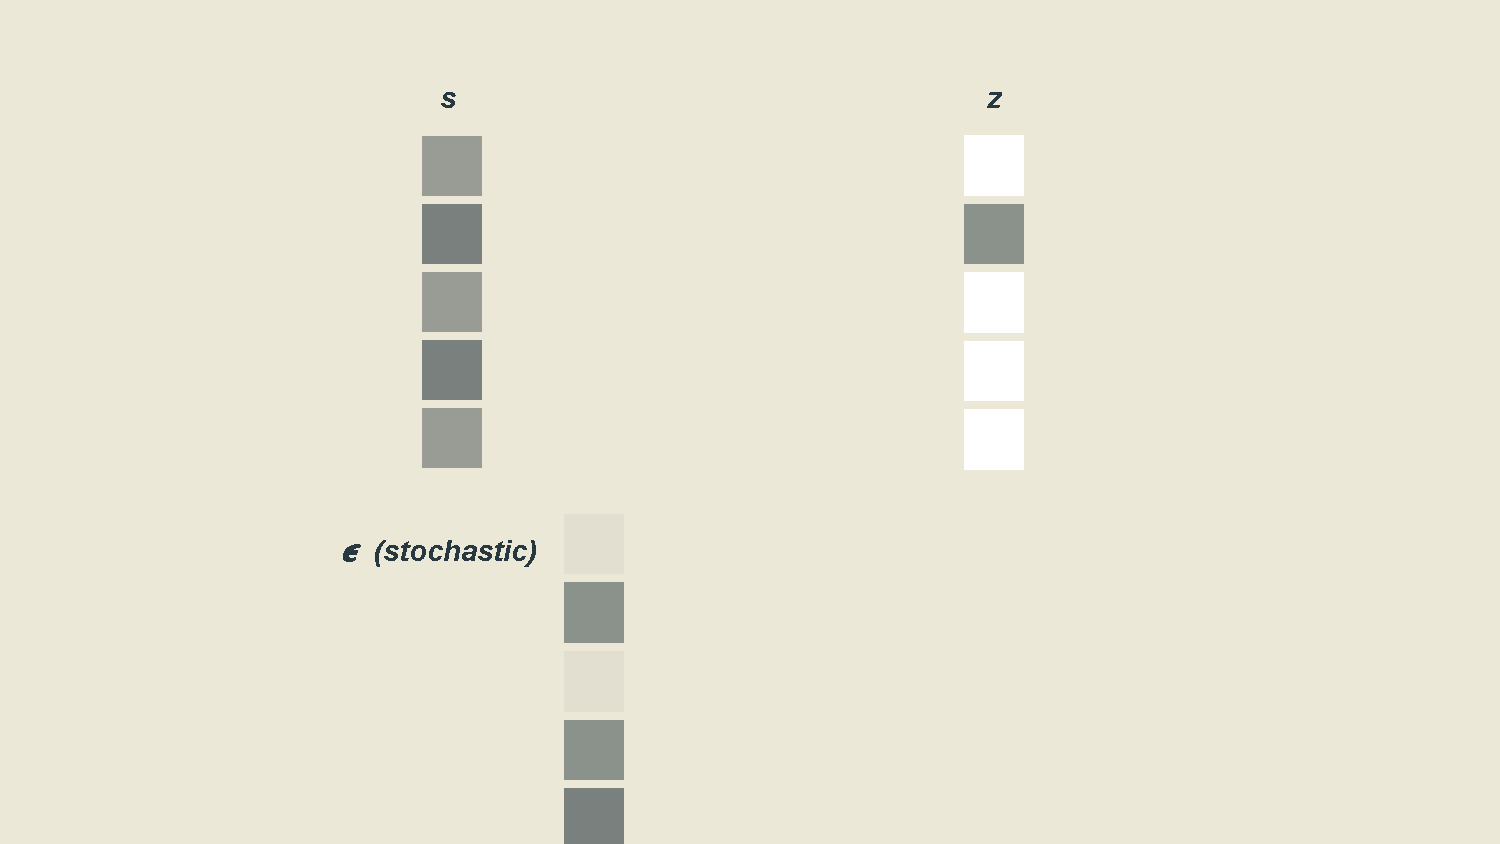
\includegraphics[width=\textwidth]{img/300_reparam_2.pdf}}
\only<5>{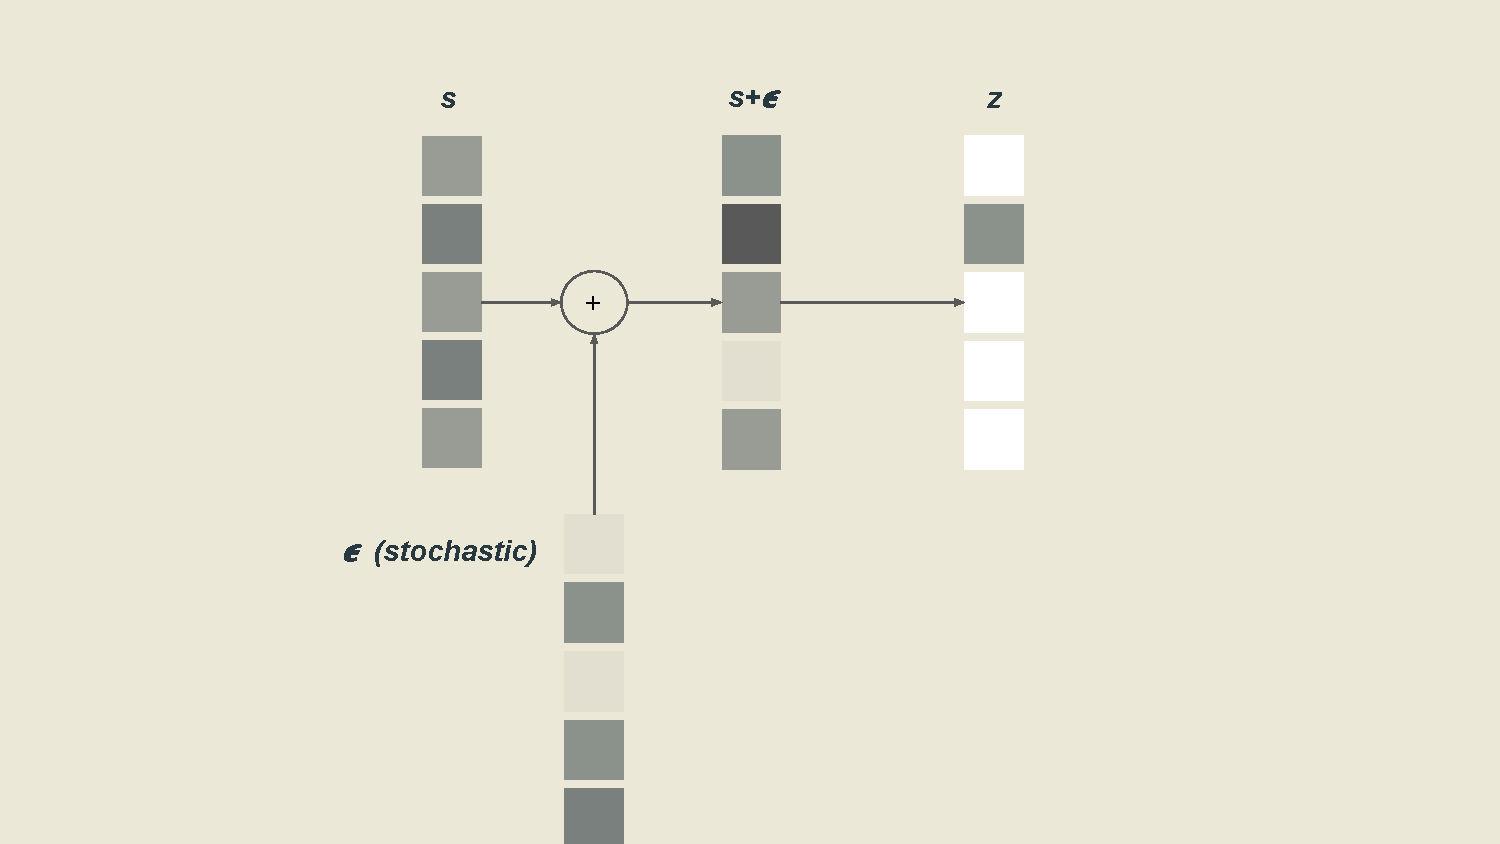
\includegraphics[width=\textwidth]{img/300_reparam_3.pdf}}
\only<6-7>{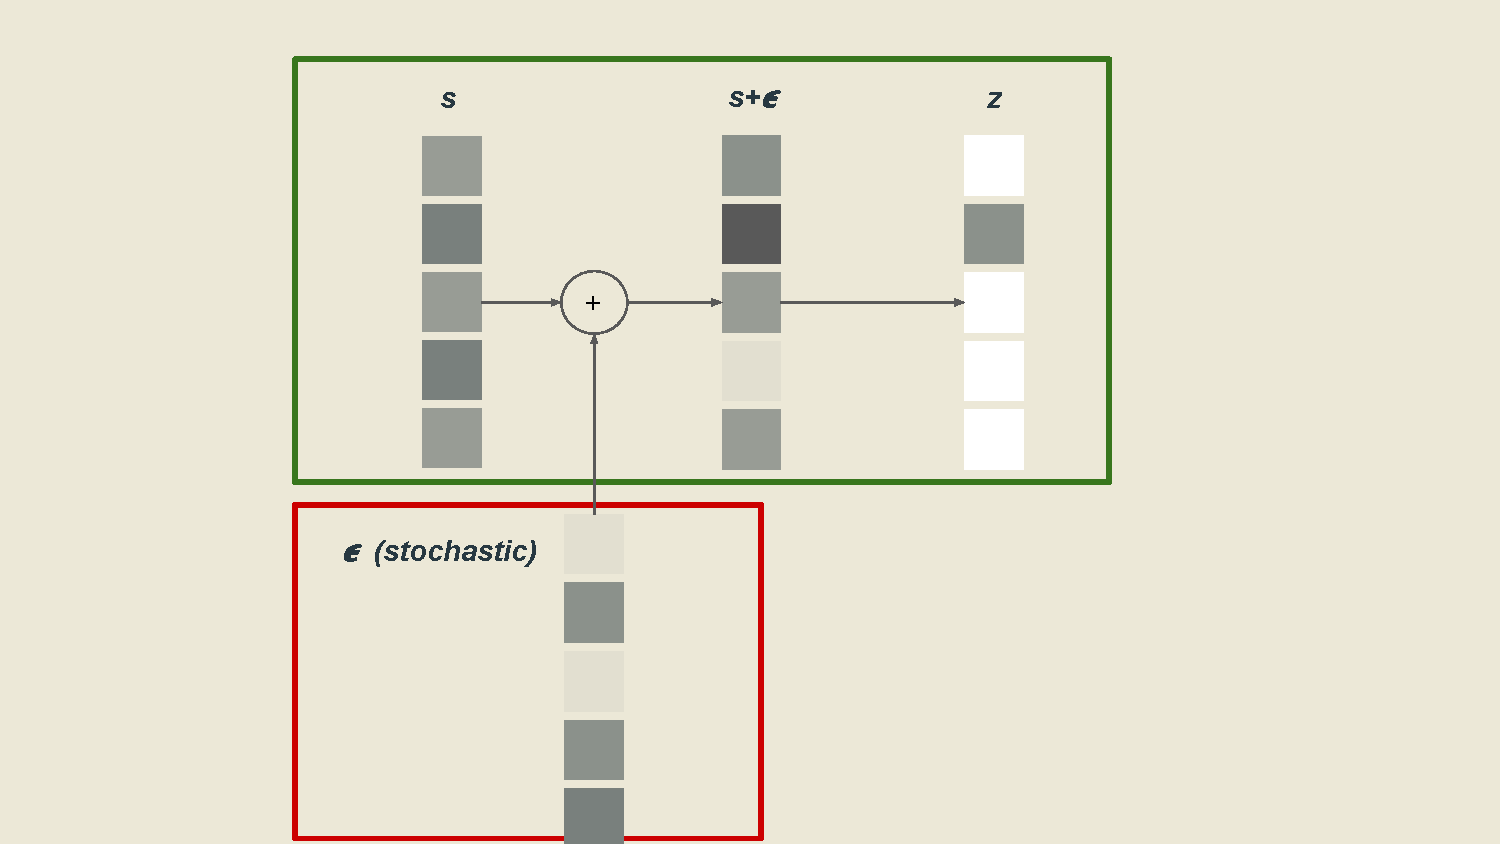
\includegraphics[width=\textwidth]{img/300_reparam_4.pdf}}
\end{column}
\end{columns}
\only<7>{\overlaybox{
\small
\underline{As a result:}\\
\small Stochasticity is moved as an input. \\
\small We can backpropagate through the deterministic input to $\z$.
}
}
\end{frame}


\begin{frame}%
\frametitle{Categorical reparameterization}%
\cornercite{jang2016categorical, maddison2016concrete}
\centering
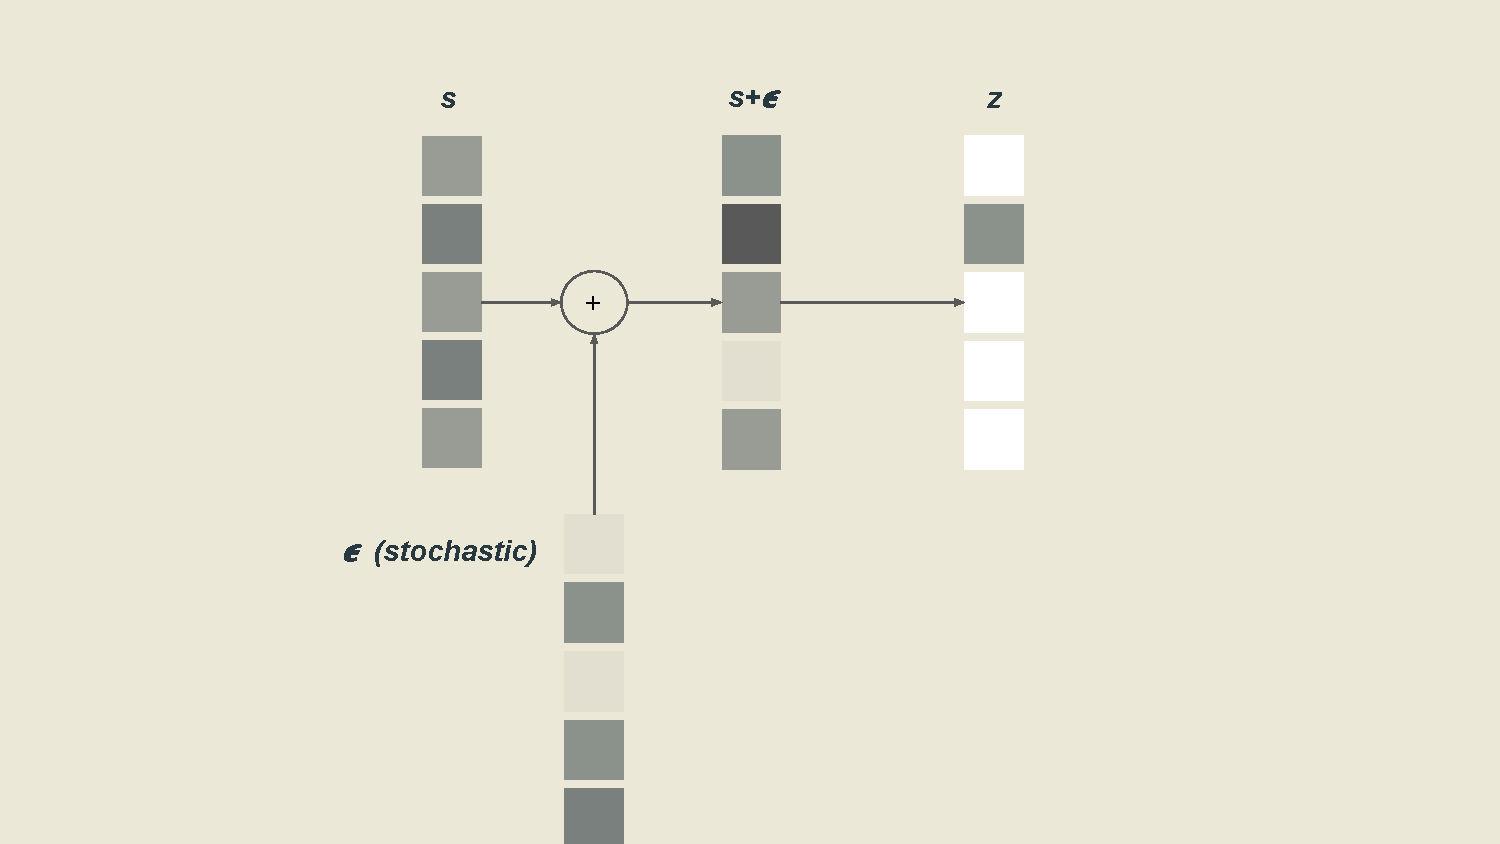
\includegraphics[width=0.8\textwidth]{img/300_reparam_3.pdf}%
\uncover<2->{\overlaybox{How do we sample from a categorical variable?}}
\end{frame}


\begin{frame}%
\frametitle{Sampling from a categorical variable}%
\framesubtitle{\small We want to sample from a categorical variable
    with scores $\s$ (class $i$ has a score $\ss_{i}$)}
\begin{columns}[t]%
\begin{column}{.5\textwidth}%
\centering%
\uncover<2->{\textbf{1. Inverse transform sampling:} \\}
\begin{itemize}
    \item<3-> $\p = \softmax(\s)$
    \item<4-> $c_{i} = \sum_{j \leq i} \pp_{j}$
    \item<5-> $u \sim \operatorname{Uniform}(0, 1)$
    \item<6-> return $\z = \bs{e}_t$ s.t.\ $c_{t} \leq u < c_{t+1}$
\end{itemize}
\end{column}
\begin{column}{.5\textwidth}%
\centering%
\uncover<7->{\textbf{2. The Gumbel-Max trick} \\}
\begin{itemize}
    \item<8-> $u_i \sim \operatorname{Uniform}(0, 1)$
    \item<9-> $\epsilon_{i} = -\log(-\log(u_i))$
    \item<10-> $\z = \argmax(\s + \bs{\epsilon})$
\end{itemize}
\end{column}
\end{columns}
\vspace{\baselineskip}
\centering
\uncover<11->{\small{The two methods are equivalent. \textit{(Not obvious, but we will not prove it now.)}}\\}
\uncover<12->{\small{Requires sampling from the Standard Gumbel Distribution G(0,1).}\\}
\uncover<13->{\small\textit{Derivation \& more info:
\citep{ryanadamsblog,timblog}}}
\uncover<14->{\overlaybox{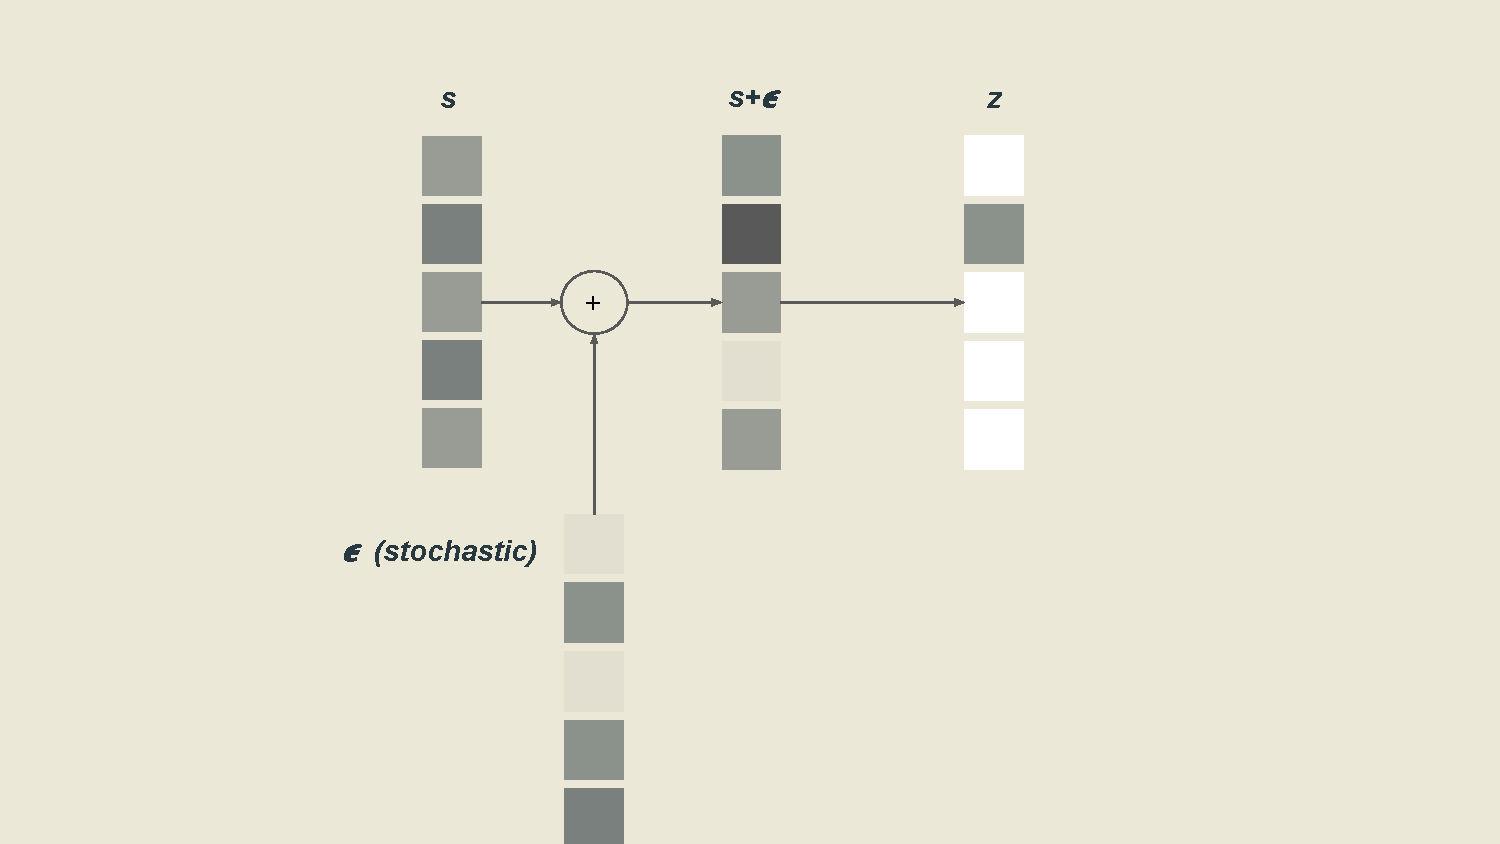
\includegraphics[width=.6\textwidth]{img/300_reparam_3.pdf}}}
\uncover<15->{\overlaybox{We have an argmax again\\
    and cannot backpropagate!}}
\end{frame}



\begin{frame}%
\frametitle{Straight-Through Gumbel Estimator}%
\framesubtitle{\small Apply a variant of the Straight-Through Estimator to Gumbel-Max!}
\cornercite{jang2016categorical, maddison2016concrete}
\centering
\begin{columns}[T]
\begin{column}{.4\textwidth}
% \small
\begin{itemize}
    \item<2->Forward: % $argmax$\\
    $\z = \argmax(\s + \bs{\epsilon})$
    \item<3->Backward: pretend we had done \\
    $\tilde\p = \softmax(\s + \bs{\epsilon})$
\end{itemize}
\end{column}
\begin{column}{.6\textwidth}
\only<2>{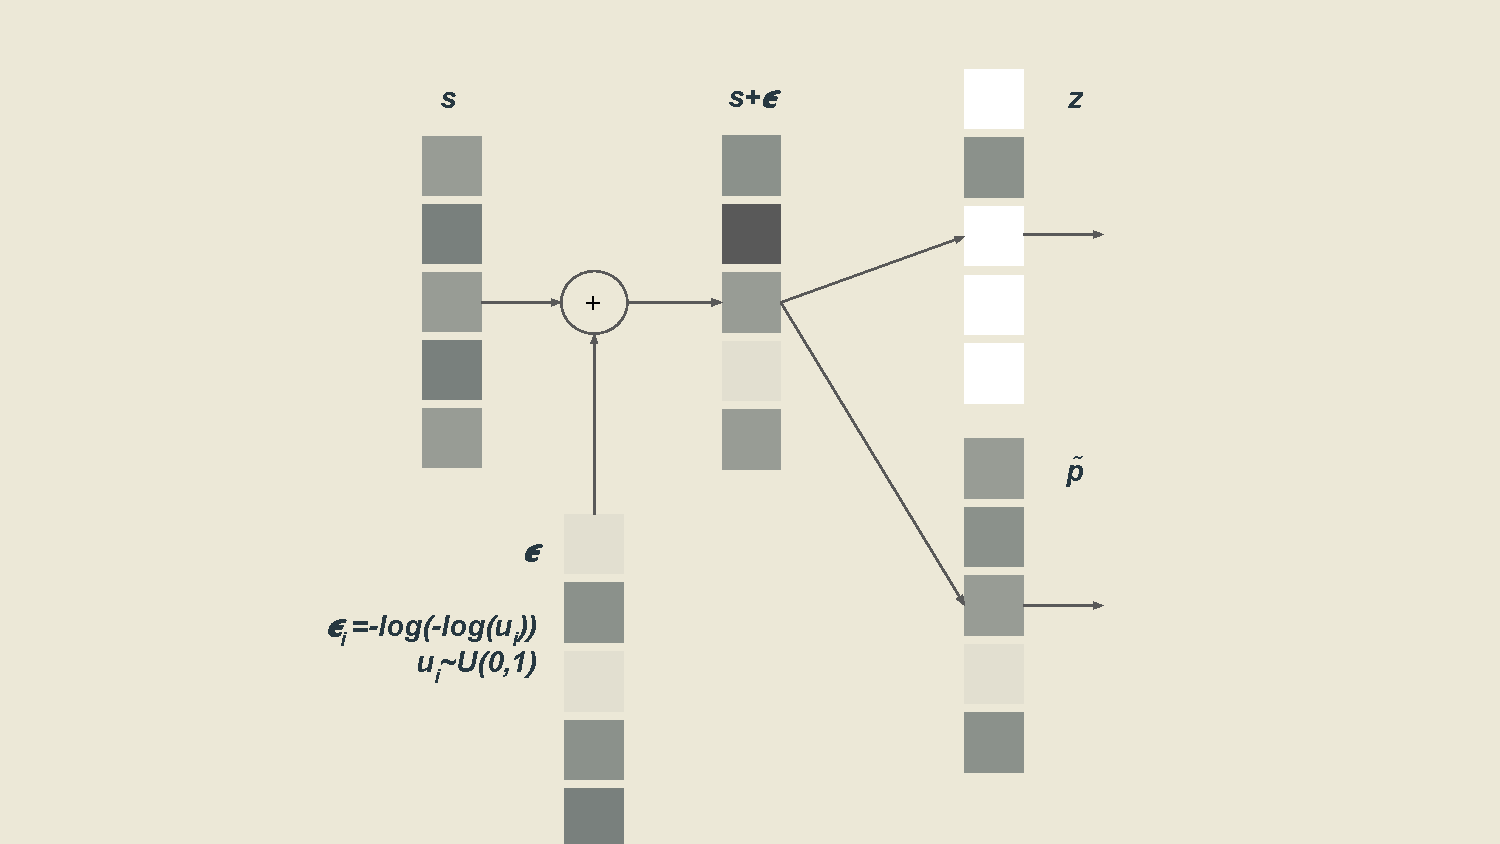
\includegraphics[width=\textwidth]{img/300_reparam_gumbel_st.pdf}}
\only<3-4>{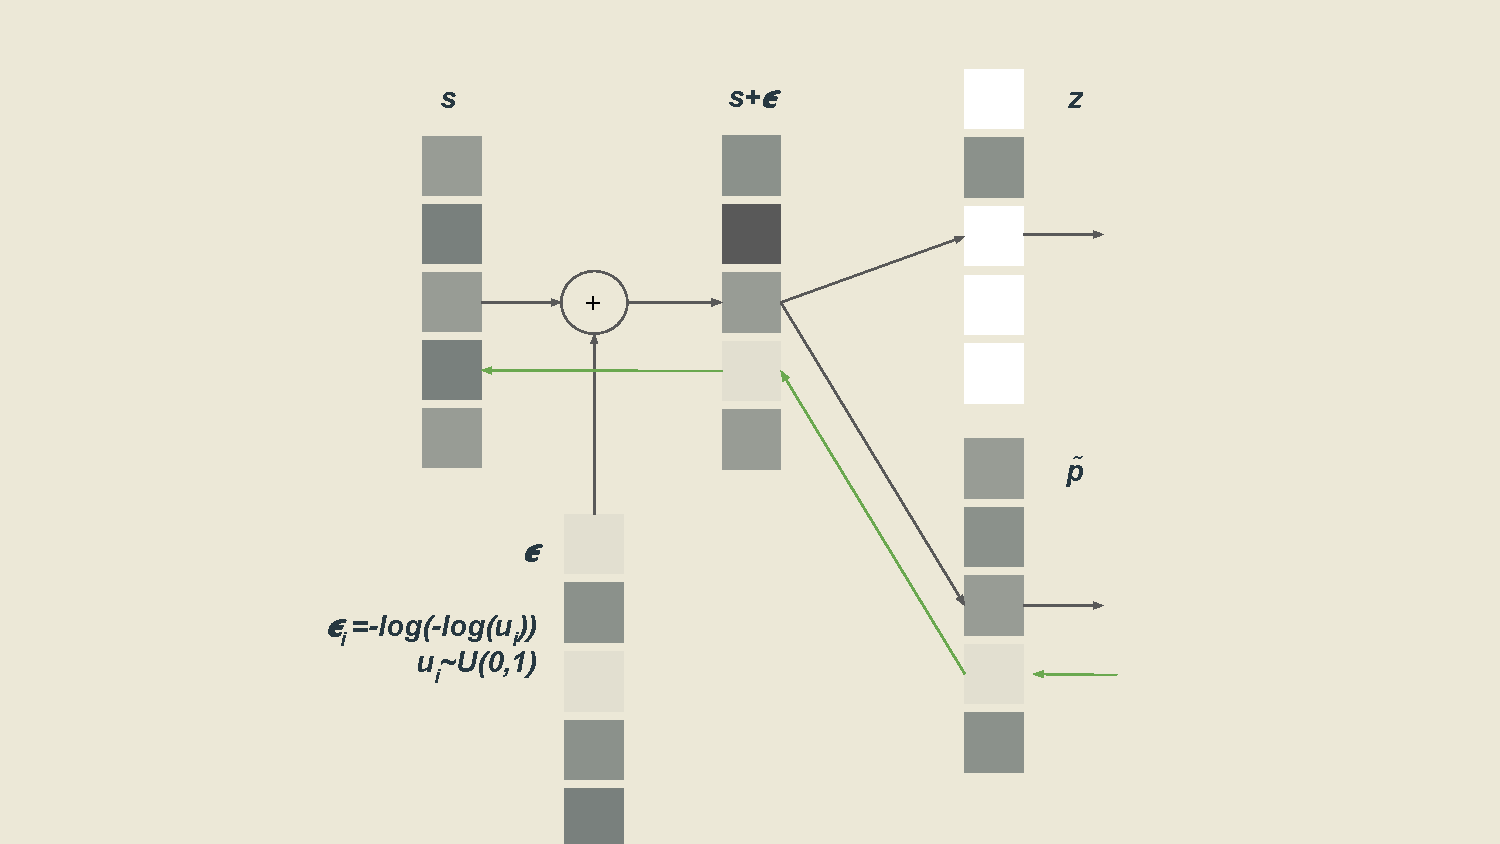
\includegraphics[width=\textwidth]{img/300_reparam_gumbel_st_back.pdf}}
\end{column}
\end{columns}
\uncover<4->{\overlaybox{What about the structured case?}}
\end{frame}


\againframe{structuretypes}


\begin{frame}%
\frametitle{Sampling from incremental structures}%
\centering
\begin{itemize}
    \item<2-> Build a structure as a sequence of discrete choices (e.g., shift-reduce)
    \item<3-> Assigns a score to any (partial structure, action) tuple.
    \item<4-> Reparameterize the scores with Gumbel-Max - now we have a deterministic node.
    \item<5-> \underline{Forward}: the \textbf{argmax} from the reparameterized scores for each step
    \item<6-> \underline{Backward}: pretend we had used a \textbf{differentiable surrogate function}
    \item[]<7-> \underline{Example}: Gumbel Tree-LSTM \citep{choi2017learning}.
\end{itemize}
\end{frame}


\begin{frame}%
\frametitle{Example: Gumbel Tree-LSTM}%
\cornercite{choi2017learning}
\centering
\small
\begin{itemize}
\item Building task-specific tree structures.
\item Straight-Through Gumbel-Softmax at each step to select one arc.
\end{itemize}
\begin{center}
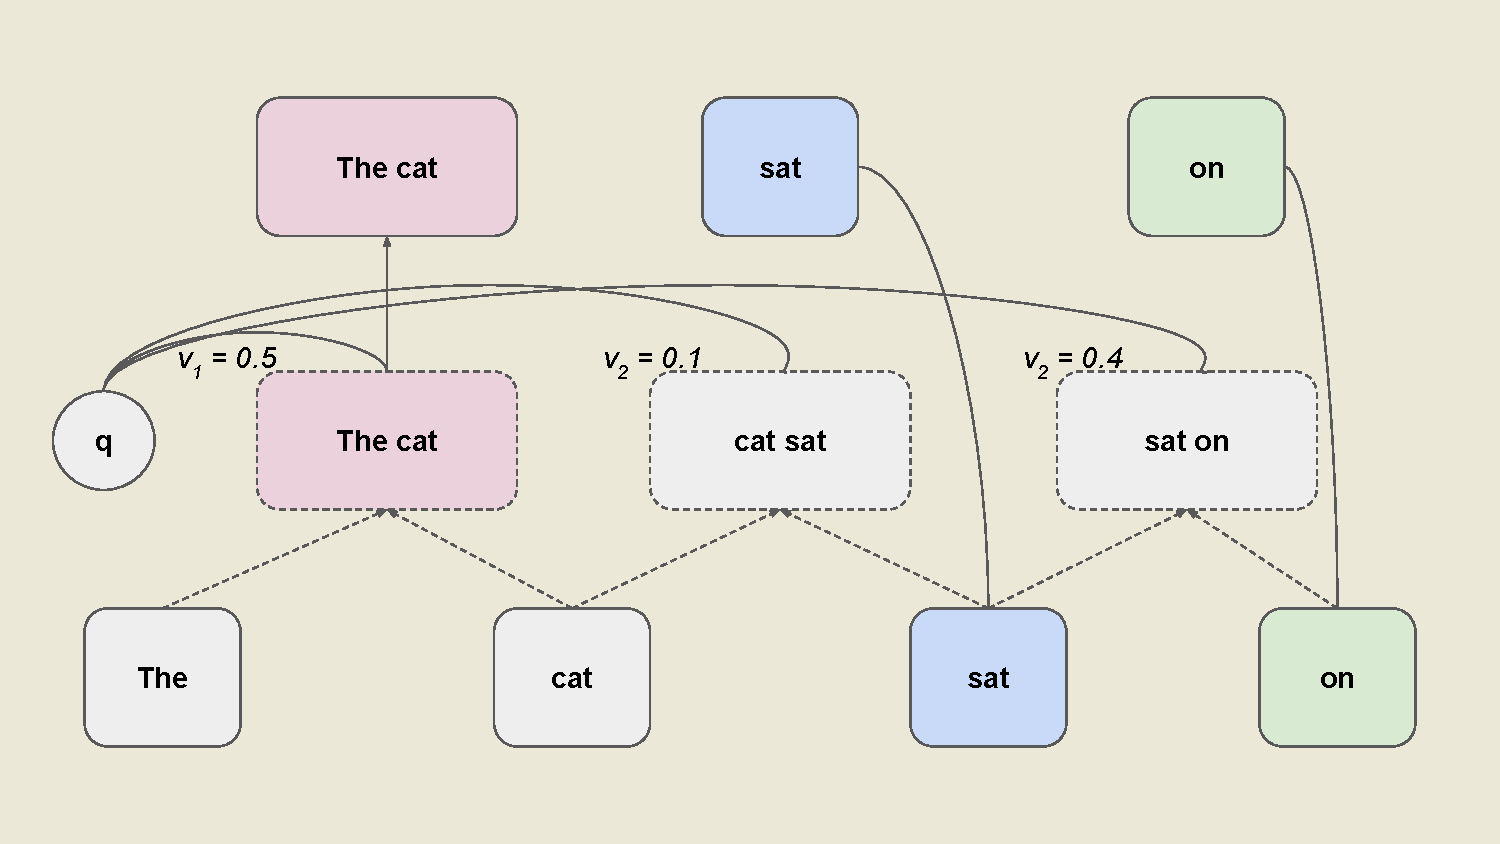
\includegraphics[width=0.6\textwidth]{img/300_gumbel_tree_lstm.pdf}%
\end{center}
\end{frame}



\begin{frame}%
\frametitle{Sampling from factorized models}%
\framesubtitle{Perturb-and-MAP}%
\cornercite{perturbandmap,corro2018differentiable,corro2019acl}
\centering
Reparameterize by \textbf{perturbing the arc scores}.
(inexact!)
\\[\baselineskip]
\begin{columns}[t]%
\begin{column}{.6\textwidth}%
\centering%
\begin{itemize}
    \item<2-> Sample from the normal Gumbel distribution.
    \item<3-> Perturb the arc scores with the Gumbel noise.
    \item<4-> Compute MAP (task-specific algorithm).
    \item<5-> Backward: we could use Straight-Through with Identity.
\end{itemize}
\end{column}
\begin{column}{.4\textwidth}%
\centering%
\begin{itemize}
    \item<2-> $\bs{\epsilon} \sim G(0,1)$
    \item<3-> $\tilde \pr = \pr + \bs{\epsilon}$
    \item<4-> $\argmax_{\z \in \ZZ} \tilde \pr ^\top \z$
\end{itemize}
\end{column}
\end{columns}
\end{frame}


\begin{frame}%
\frametitle{Summary: Gradient surrogates}%
\centering
\begin{itemize}
    \item Based on the \textbf{Straight-Through Estimator}.
    \item Can be used for stochastic or deterministic computation graphs.
    \item \textbf{Forward pass}: Get an argmax (might be structured).
    \item \textbf{Backpropagation}: use a function, which we hope is close to argmax.
    \item Examples:
        \begin{itemize}
            \item Argmax for iterative structures and factorization into parts
            \item Sampling from iterative structures and factorization into parts
        \end{itemize}
\end{itemize}
\end{frame}

% \begin{frame}%
% \frametitle{Examples: Gradient Surrogates}%
% \centering
% \begin{itemize}
%     \item Deterministic case.
%     \begin{itemize}
%         \item Identity on the backward pass. %\citep{corro2019acl}.
%         \item Marginals on the backward pass. %\citep{corro2019acl}.
%         \item SPIGOT (\citep{peng2018backpropagating})
%         \item Differentiable shift-reduce parsing (\citep{maillard2018latent}).
%     \end{itemize}
%     \item Examples for sampling latent structures.
%     \begin{itemize}
%         \item Perturb-and-MAP (\citep{corro2018differentiable}): Imitate sampling a tree by perturbing arc scores (an approximation of the real distribution.)
%         \item Gumbel Tree-LSTM (\citep{choi2017learning}):  Sample one action iteratively.
%     \end{itemize}
% \end{itemize}
% \begin{tabular}{l l{1in} l{1in}}
%     \small
%      & Deterministic & Stochastic \\
%     Iterative & Differentiable shift-reduce \citep{maillard2018latent} & Gumbel-TreeLSTM \citep{choi2017learning} \\
%     Factorized & SPIGOT \citep{peng2018backpropagating} & Perturb-and-Parse \citep{corro2018differentiable} \\
% \end{tabular}
% \end{frame}

\begin{frame}%
\frametitle{Gradient surrogates: Pros and cons}%
\centering
Pros
\begin{itemize}
    \item Do not suffer from the high variance problem of REINFORCE.
    \item Allow for flexibility to select or sample a latent structured in the middle of the computation graph.
    \item Efficient computation.
\end{itemize}
Cons
\begin{itemize}
    \item The Gumbel sampling with Perturb-and-MAP is an approximation.
    \item Bias, due to function mismatch on the backpropagation\\\quad(next section will address this problem.)
\end{itemize}
\end{frame}

\begin{frame}<1-2>[t,label=overview]%
\newcommand{\samp}{\textcolor{tPink}{\scriptsize SPL}}
\newcommand{\map}{\textcolor{tGreen}{\scriptsize MAP}}
\newcommand{\marg}{\textcolor{tBleu}{\scriptsize MRG}}
\setbeamertemplate{itemize/enumerate body begin}{\small}
\frametitle{Overview}%
\begin{columns}[T]%
\begin{column}{.333\textwidth}
\centering
$$\EE_{\parser}\big[L(\z)\big]$$
\begin{itemize}
\item REINFORCE\only<6->{\textsuperscript{\samp}}
\item Straight-Through Gumbel\\ \quad (Perturb \& MAP)%
\only<6->{\textsuperscript{\samp,\marg}}
\item<5-> SparseMAP\only<6->{\textsuperscript{\map{}+}}
\end{itemize}
\end{column}
\begin{column}{.333\textwidth}
\centering
$$L\big(\textstyle \argmax_z \parser\big)$$
\begin{itemize}
\item Straight-Through\only<6->{\textsuperscript{\map,\marg}}
\item SPIGOT\only<6->{\textsuperscript{\map{}+}}
\end{itemize}
\end{column}
\onslide<2->{%
\begin{column}{.333\textwidth}
\centering
$$L\big(\EE_{\parser}[\z]\big)$$
\begin{itemize}
\item<2,4-> Structured Attn. Nets\only<6->{\textsuperscript{\marg}}
\item<2,4-> SparseMAP\only<6->{\textsuperscript{\map{}+}}
\end{itemize}
\end{column}}
\end{columns}
%\only<4-5>{%
%\centering \small \textbf{Model restrictions:}\\
%\begin{columns}[T]%
%\begin{column}{.333\textwidth}
%\begin{itemize}
%\item  $\dom L$ may be only $\ZZ$,
%\item $\nabla_{\z} L$ need not exist!
%\end{itemize}
%\end{column}
%\begin{column}{.333\textwidth}
%\begin{itemize}
%\item $L(\z)$ with $\z \in \ZZ$ in forward
%\item needs (relaxed) $\nabla_{\z} L$ in backward.\\
%\end{itemize}
%\end{column}
%\begin{column}{.333\textwidth}
%\begin{itemize}
%\item $L(\z)$ must be relaxed\\ and differentiable.
%\item (sparsity gets us closer to $\ZZ$).
%\end{itemize}
%\end{column}
%\end{columns}
%}
\only<6->{%
\centering \small \textbf{Computation:}\\
\begin{itemize}
\item[] \samp{}: Sampling. (Simple in incremental/unstructured, hard for most
global structures.)
\item[] \map{}:  Finding the highest-scoring structure.
\item[] \marg{}:  Marginal inference.
\end{itemize}}
\onslide<2>{\overlaybox[.8]{And more, after the break!}}
\end{frame}
